\label{ch:methods}

This chapter is structured in the four main section, entitled \emph{SoA in embedded systems (Embedded SoA)}, \emph{SoA in automotive}, \emph{safety services} and \emph{service development process}. 

The first section deals extensively with the possible application of the service oriented design paradigm in embedded system and deals with the challenges this approach has to face when approached with safety-critical requirements. Moreover, the differences to conventional SoAs, as Web application is investigated in detail. 
The second section presents various examples of services, which are relevant for \emph{functional safety} in detail and presents their intended functionality, as well as possible implementations in terms of an architecture.

The final part consists of a simplified use case, dealing with the design of an error detection service with respect to the design phases \emph{service investigation/ planning}, \emph{service inventory analysis}, \emph{service oriented analysis} and \emph{service oriented design}.

Most of the findings and concepts in this chapter are (not yet) covered in literature, but is the result of numerous meetings and discussions at VIRTUAL VEHICLE during May to July 2015.









\section{SoA in Embedded Systems (Embedded SoA)}
\label{sec:soa-in-embedded-systems}

The service oriented design paradigm was originally designed for the application in the web, which offered ideal prerequisites for this kind of architectural style: An underlying network for interconnection is already present and \emph{time constraints} are no concern, for delays are unlikely to cause a disaster. Thus, it is no surprise that web services are the application area, where SoA has scored the highest market penetration \cite{rodrigues2011} \cite{buckl}.


\subsection{Drawbacks in embedded systems}
In contrast to web services, \emph{embedded systems} consist of numerous interconnected nodes, with diverse measurement-, steering-, or computation capabilities. They have to face additional challenges like \emph{limited resources}, \emph{different complexity of hardware}, \emph{time constraints}, etc. \cite{scholz} \cite{sommer}. 

The most crucial of those obstacles are investigated in more detail in the following.

\begin{description}
\item [Limited resources].
One obvious major drawback of embedded systems are the quite limited resources, which are designed for highly specialized purposes and lack computation power as well as storage size \cite{rodrigues2011} \cite{scholz} \cite{sommer}.

\item [Different levels of complexity].
The complexity of hardware varies greatly. The applied components may include very primitive sensors, with few capabilities and very advanced nodes like MPSoCs, at the same time \cite{scholz} \cite{sommer}.

In other words, there are high level \emph{information systems services}, as well as low level generic \emph{embedded system services}. It is the task of SoA to deal with the connection and integration of them \cite{rodrigues2011}. This task gets aggrevated if SoAs in embedded systems are connected to high level SoAs like web applications.

\item [Event- and data-driven].
In contrast to web services, an embedded system disposes of a network with (many) sensors. Thus, the ad-hoc \emph{request-response} message pattern, which is common for web services, cannot be simple addopted for the event- and data driven embedded systems \cite{sommer}

Instead, the communication in those works mainly by the \emph{fire and forget} scheme: A sensor measures some data and publishes it to all connected services, which have to decide on themselves, whether the received data is relevant, and how to process the received information \cite{sommer}.

\item [Lifespan of services].
Another difference to web services is the lifespan of services. While web services are used to work only a limited number of hours (or even minutes), the services in embedded systems could have application times of multiple years, or even lasting for the lifespan of the system \cite{buckl}.

\item [Dynamic character]. 
The components of a SoA show dynamic characteristics: \emph{``new nodes may enter the network, existing nodes may fail and network characteristics can change over time, especially if wireless communication media are used''} \cite{sommer}. This can become an issue, for conventional embedded systems dispose of a predefined set of components, which are determined when the system is assembled.

\item [Time constraints].
Embedded systems are \emph{time-critical}, meaning that computation must be conducted within a given time window in order to allow the correct operation of the system. Especially, in a safety-critical system like a vehicle, which is used to operate at high velocities, a violation of those time constraints could cause serious incidents.
\end{description}


These obstacles are the reason why web services and safety-critical embedded systems are often considered as non-related areas \cite{rodrigues2011}. Nevertheless, the application of the service oriented architecture style in embedded systems offers numerous benefits: 
\begin{itemize}
\item Decoupling configuration from environment, 
\item Improvement of reusability,
\item Improvement of maintainability,
\item Higher level of abstraction,
\item Enhanced interoperability and
\item More interactive interfaces between devices and information system \cite{buckl}.
\end{itemize}

To sum up, the SoA paradigm offers a promising approach to overcome many of embedded systems related drawbacks \cite{buckl} \cite{sommer}. Accordingly, there have been various projects dedicated to investigation of the applicability of SoA for embedded systems. Those include SIRENA, SOCRATES, OASiS, MORE, RUNES and $\varepsilon$SOA. 



\subsection{Embedded SoA}
There is no unified denomination for SoAs in embedded systems throughout literature. Thus, it is referred to by the term \emph{Embedded SoA (abbreviated as ESoA)} within this document.

The following definition is the result of our findings:
\begin{myquote}
The Embedded SoA works at a lower, very hardware oriented level, with a predefined and unchanging set of component.

The conventional SoA is located above the embedded SoA and connected through various interfaces.
\end{myquote}

With respect to the example of a vehicle, the ESoA operates on elements like a power-train, various devices (sensors, actuators, controllers, etc.), while the SoA level contains the vehicle as overall system, but also other vehicles, which can be referred to as the \emph{System of Systems}.

Regarding the ISO 26262 standard, the ESoA can be related to \textbf{Part 3: Concept phase}, and the SoA to \textbf{Part 4: Product development at the system level}.


\begin{figure}[!htbp]
\centering
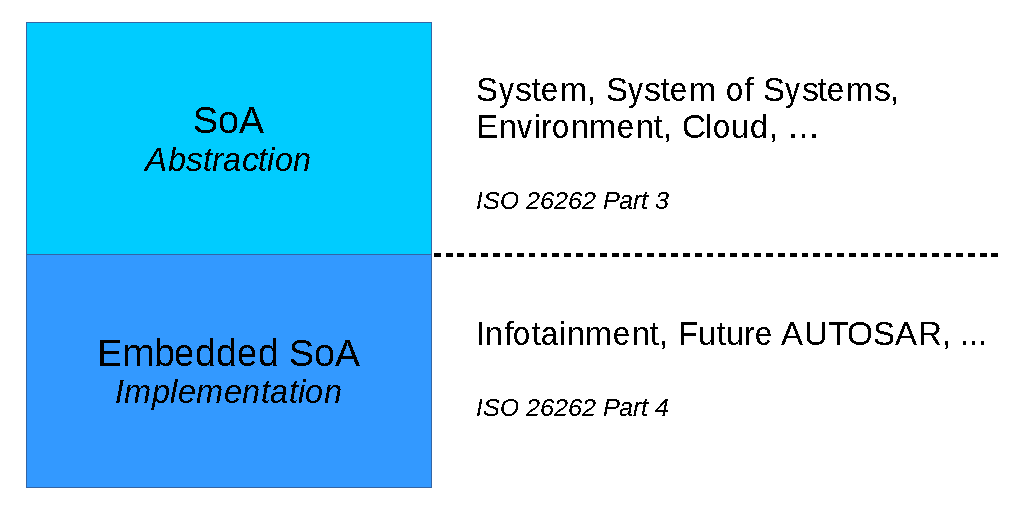
\includegraphics[scale=0.8]{soa-and-esoa.pdf}
\caption{Relation of service oriented architecture to service oriented architecture in embedded systems.}
\label{fig:soa-and-esoa}
\end{figure}







\section{SoA in automotive}
\label{sec:soa-in-automotive}

This chapter is dedicated to the investigation of the applicability of the SoA concepts for automotive.

In the future of automotive all vehicles will, most likely, be interconnected with each other and also with the environment. This could give them opportunities like automatically detecting whether the traffic lights are green at a crossing and driving autonomous. Within this document those futuristic vehicles are referred to as \emph{connected cars}.


The opportunities and advantages of the SoA approach are described extensively in \ref{sec:soa-in-embedded-systems}. In terms of vehicles, the major advantage would be the possibility to reduce the quantity of computation hardware. At present time, each component disposes of his own dedicated hardware for conducting computations, which is unused for the majority of time. Nevertheless, it comes with a lot of extra weight. As stated in \cite[p.7]{marwedel}, \emph{``Embedded systems should exploit the available hardware architecture as much as possible.s''}

The SoA approach might reduce not only the weight, but also the complexity and costs of the overall vehicle. So far, it is frequently the case that each vendor uses his own proprietary network and additional hardware, prohibiting the application of hardware components from another vendors \cite{sommer}.

Despite of all these advantages, the SoA paradigm is hardly applicable for vehicles right now. On the one hand, this is due to the strict regulations in connection with safety critical real-time systems like vehicles, where an error or a malfunction can easily harm people \cite{kum}. There are not even regulations, addressing SoA in automotive, yet.

On the other hand, there are technical constraints. The AUTOSAR architecture, which is widely applied today, is not constructed for dynamic reconfiguration or binding of services, but everything has to be specified at building time. Still, there is already an approach by AUTOSAR, denoted ``Future AUTOSAR'', which is dealing with this very issue.

Although, the SoA for vehicles is still a long way ahead, it might be easier applicable at a higher level, like at the \emph{system of systems} level (other vehicles and the overall traffic). For example services for the communication with traffic lights or other participants of the traffic. If the the traffic lights in Germany would use another service as the ones in Austria, a SoA could enable the dynamical binding of the new service, when the border is approached. There are already dedicated projects which are dealing with the communication between vehicles.


\subsection{Location of the service repository}
The terms service repository is already covered in detail in the related glossary. Nevertheless, questions arose concerning its location and actual implementation with respect to automotive. This section covers the findings concerning this matter.
\\
\\
For SoAs in automotive it is likely that there will emerge various distributed repositories. One repository inside of every vehicle, containing all the services provided by the vehicle itself, which is also available if the vehicle is operating in urban regions and is not able to connect to its environment. For the SoA inside the vehicle, there is no other possible location, because otherwise it would be operable only as long as it is connected to the Internet, or whatever platform, which is used for the interconnection with the environment.

For the scope of this document these repositories will be referred to by the term \emph{local service repository}. Examples for the services they hold are services which origin from hardware components of the vehicle like, acceleration measurement, temperature measurement, communication services and the like. But also safety critical services for fault- and error detection, which need to be available whenever the vehicle is operated, are located within this repository.

The counterpart to the \emph{local service repository} is denoted \emph{external service repository}. This could also be physically distributed and holds mostly services which are needed for interacting with the environment. For ``self-driving-'' or ``connected cars'' it could host all the services for managing the traffic. For example: A traffic light in Graz publishes its service, ``Show me the traffic light signal'', somewhere on a server, where it is detected and bound by a vehicle driving in Graz. It is then able to decide automatically whether it has to stop at an intersection.

Other services which could be located in this repository are \emph{update services}. If an update for an existing service in the local repository is available, the vehicle could detect this automatically and subsequently load and install the service in question.


\subsection{Service Contract}

The service contract is the complete and extensive description of the service and should contain (with regard to vehicles) documents from AUTOSAR, the ISO 26262 standard and documentation regarding \emph{functional safety}. It is one of the goals of \textbf{Work Package 1} of the EMC2 project to extend the \emph{service contract} by a functional safety part.

At the beginning of a service development process, the contract exists just as an empty template, which gets filled more and more as the development advances. A template, which could be used for the development of services in the automotive industry is already provided by the ARROWHEAD project.








\section{Safety services}

If safety-critical systems, like vehicles, get connected to the outside world, security becomes an important issue and most of the provided services must be fault tolerant and secure at the same time.

There are many challenges for safety and security management in SoA systems, like the distributed hardware and software structure, loosely coupled components from different vendors, etc.

\emph{Functional safety} is directly related to \emph{availability} and thus the overall safety can be increased by increasing the availability \cite{turek2011}. According to \cite{turek2011}, a system has to generate the correct output in order to be available. Services for failure detection, error detection and error masking can increase the availability and also enable recovery from errors.

In the following sections, the interference and connection of safety and security services is analysed, before the principles of some of a few selected safety services is investigated in more detail.

\subsection{Relation of Safety and security services}

As described in the glossary, in vehicles it is not possible to distinguish between safety functions and ``normal'' functions, because vehicles operate at high velocities and a failure of any functionality could lead to a disaster \cite{iso26262:course2}. Therefore, all services are considered safety-critical.

Since future vehicles are planed to be always connected to the outside world, \emph{security} must also be taken into account, because a malicious attack on the system could be equally disastrous. Accordingly, all services must also take a security aspect in consideration. Comparable to functional safety and fault tolerance, security will be taken care of by dedicated services.

However, some services cannot be assigned to any of the disciplines, but have overlapping responsibilities, as depicted in figure \ref{fig:safety-and-security-services}. According to our findings this effects especially the services for \emph{authentication}, \emph{memory protection} and \emph{failure detection}.s

\begin{figure}[!htbp]
\centering
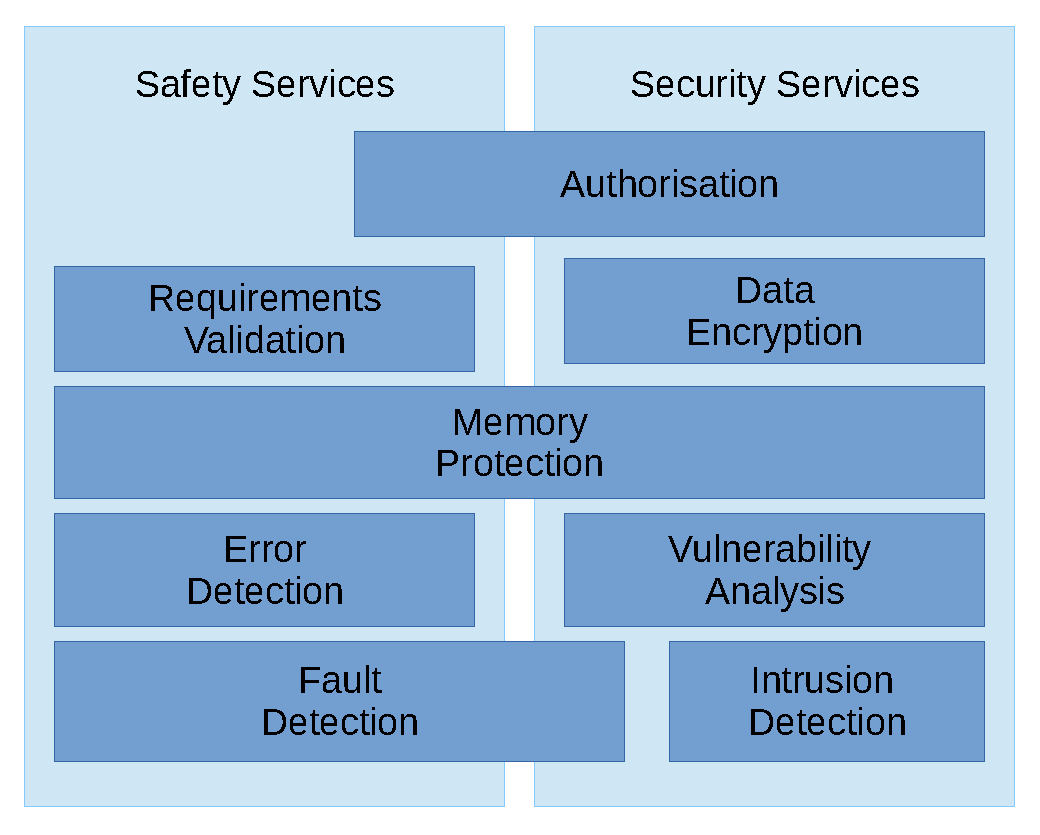
\includegraphics[scale=0.6]{safety-and-security-services.pdf}
\caption{Classification of various services into safety and security services.}
\label{fig:safety-and-security-services}
\end{figure}




\subsection{Failure detection service}

A Fault Detection Service (FDS) is a service which is capable of detecting faults, and eventually, depending on its implementation, also \emph{control flow errors}. Control flow errors are errors, which lead to a wrong execution sequence of the instructions of a service.
Technically, the FDS can be implemented as simple timer circuit with a specified threshold time. If this limit is reached, it changes its state for triggering further actions, like restarting a component or activating another safety service [7].
The advantages of the FDS are the simple design, which reduces the additional complexity of the overall system, as well as the costs. Concerning the functional principle, there different designs with increasing complexity, which can provide, for example, a certain time window for the response [7].


\begin{figure}[!htbp]
\centering
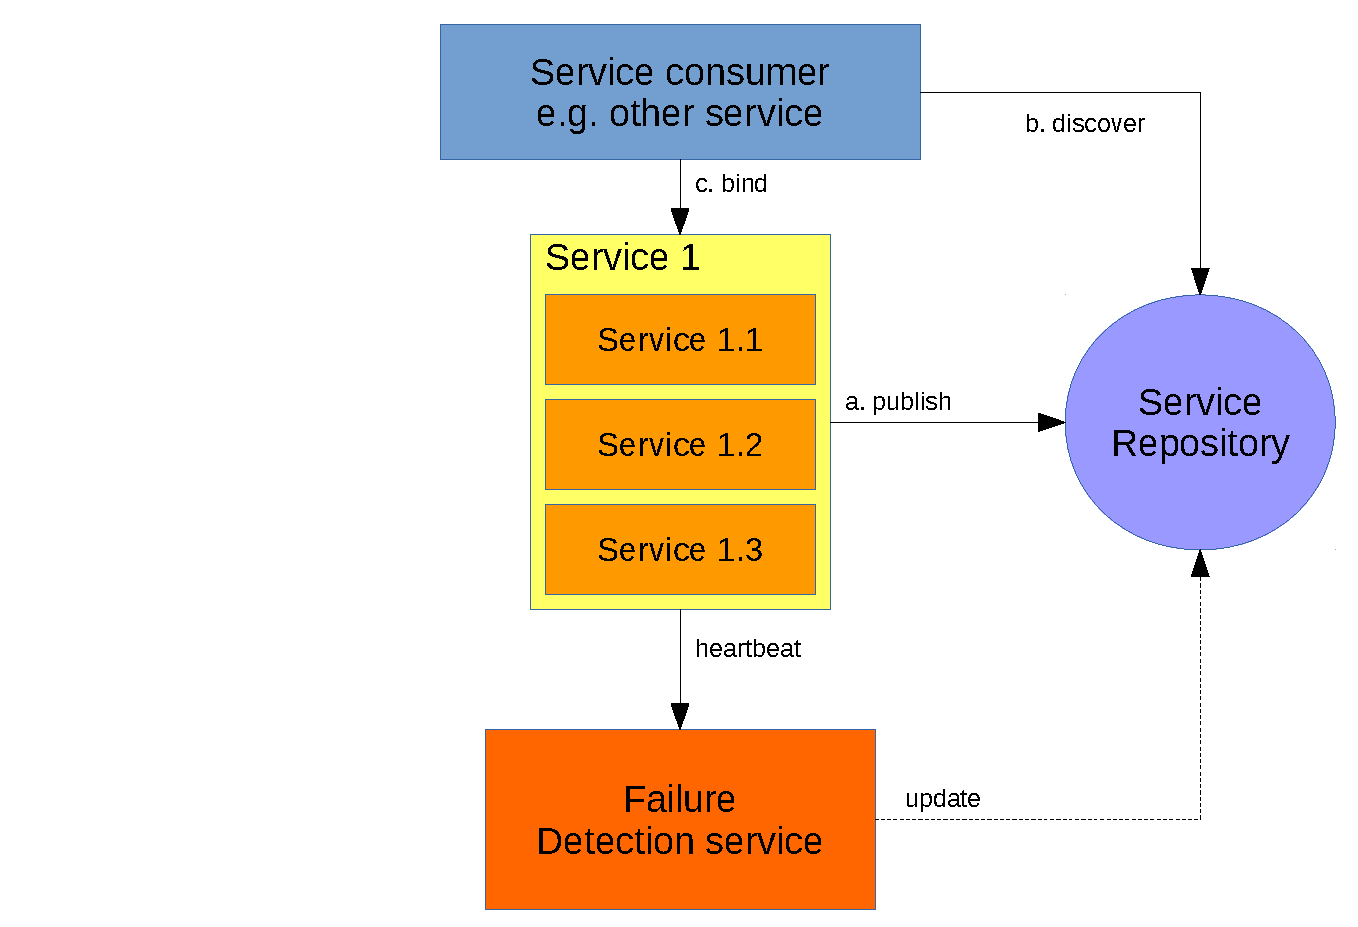
\includegraphics[width=\textwidth]{fault-detection-service.pdf}
\caption{Example architecture for an \emph{fault detection service}, like a WDT.}
\label{fig:fault-detection-service}
\end{figure}

In the following, a fault detection service is described by means of its most prominent representative, the so called \emph{Watchdog Timer}.
\\
\\
As suggested by the name, the WDT is based on a timer, which gets reset every time, a heartbeat signal from the observed service is received. There three different basic designs: the \emph{Standard Watchdog Timer}, the \emph{Windowed Watchdog Timer} and the \emph{Sequenced Watchdog Timer} \cite{elattar2007}.


\begin{description}
\item [Standard Watchdog Timer] .
With this basic setup, the service mirrored by the WDT periodically sends a simple heartbeat signal, indicating that the service is alive and active. This signal resets the timer. It a predefined amount of time elapsed, without an incoming signal, it is assumed that a fault has occurred and the WDT changes its state \cite{elattar2007}.

In terms of \emph{control flow errors} in a service, the heartbeat signal may, or many not, be sent too late. In the latter case, the WDT is capable of detecting the error \cite{elattar2007}. 
The probability of noticing such an error is higher, the closer the threshold time is to the time between the heartbeat signals.

\item [Windowed Watchdog Timer] .
The \emph{Windowed Watchdog Timer} is an improvement of the standard version, which is capable of detecting most of the \emph{control flow errors}. This is enabled by the application of two timers instead of one. With two timers the WDT is able to specify a time window, during which the heartbeat signal from the observed service must be received. The WDT is triggered if it receives a signal outside the window, or the timer reaches its threshold \cite{elattar2007}. This is illustrated in figure \ref{fig:windowed-watchdog-timer} with the $time$ on the x-axis and the Timers labeled $T1$ and $T2$.

In case of an \emph{control flow error} this signal is a bit ahead or past in time. The error detection coverage increases with narrowing the time window \cite{elattar2007}.  

The advantage of this design is clearly that it allows the detection of more errors, but on the other hand the implementation is slightly more complex.

\begin{figure}[!htbp]
\centering
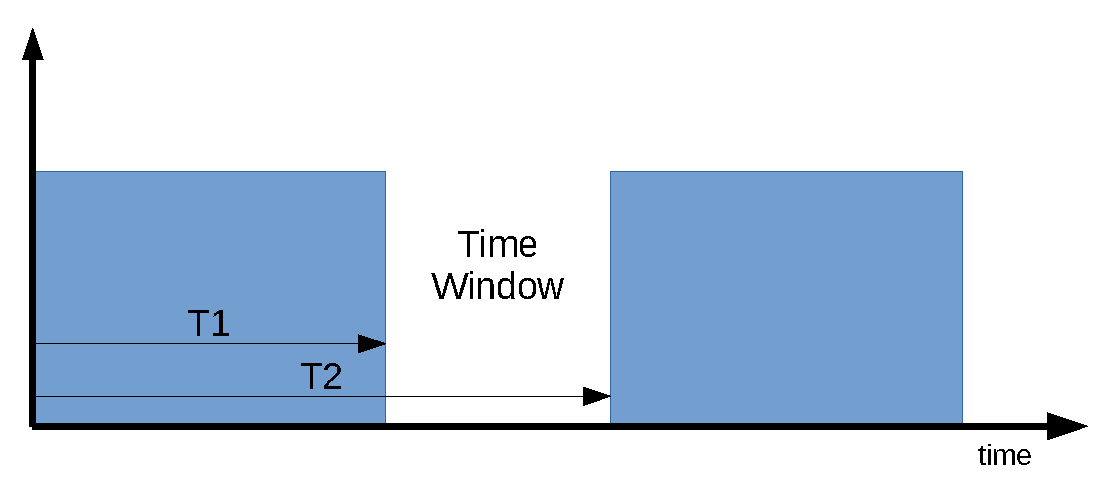
\includegraphics[scale=0.6]{windowed-watchdog-timer.pdf}
\caption{Schematic design of a windowed watchdog timer \cite{elattar2007}. The time windows is the result of $T2 - T1$.}
\label{fig:windowed-watchdog-timer}
\end{figure}

\item [Sequenced Watchdog Timer] . 
This design is a further improvement of the \emph{Windowed Watchdog Timer} and bases on the same principle. In contrast, to the other designs, the signal sent from the mirrored service carries a sequenced parameter. Only if the signal arrives in time and within the specified time window, this parameter is evaluated and compared to a parameter inside the WDT. If those match the sequence variable in the WDT is incremented and the timer reseted, starting the cycle over again \cite{elattar2007}.
The whole proce ss is illustrated in figure \ref{fig:sequenced-watchdog-timer}.

The disadvantage of this design is the clearly higher complexity, for the \emph{Sequenced Watchdog Timer} must be capable of holding and modifying state information as well as comparing it to received information.

\begin{figure}[!htbp]
\centering
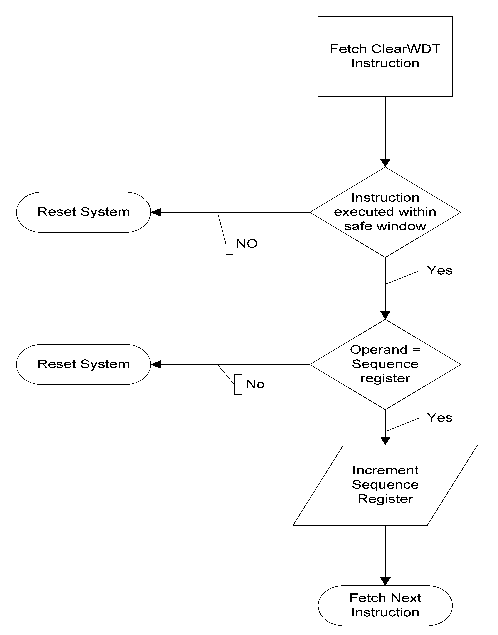
\includegraphics[scale=1.2]{sequenced-watchdog-timer.pdf}
\caption{Schematic illustration of the working process of a \emph{Sequenced Watchdog Timer} \cite{elattar2007}.}
\label{fig:sequenced-watchdog-timer}
\end{figure}

\end{description}






\subsection{Error Detection/Masking Service}
\label{sec:error-detection-service}

Most of the errors, especially those which do not alter the timing, remain unnoticed by the WDT. There are several approaches in the design of an \emph{error detection service}, but the most simple and approved one, is based on \emph{triple modular redundancy} (TMR). With this approach an \emph{error detection service} mirrors three individual and independent services, which provide the same functionality. With respect to automotive, this could be, for example, services for acceleration measurement. A comparing logic inside the \emph{error detection service} compares the information received from these services and can identify an error in one of the services by means of a simple voting mechanism \cite{wiki_tmr}.

In advance, another service can be triggered for restarting the service in question, or other actions.

The very same implementation is also capable of performing \emph{error masking}, because due to the redundancy and the voting system the service could also hide an error in one of the mirrored elements, without the service consumer noticing.


\subsection{Memory Protection}
\emph{Memory protection} is related to \emph{safety} as well as \emph{security}. It is a method for preventing processes or users from accessing memory that is not allocated to them.

Former embedded systems, or such that are small in size, do not necessarily require memory protection mechanisms, because all related programs have a very specific purpose and an unintended behaviour is rather unlikely. In such cases the overhead in runtime, when using memory protection just does no pay off \cite{yamada2008}. 

However, modern, large scale system, have numerous third-party components are used to interact with the user and the environment. At the same time, the overhead in computing is no longer crucial, due to the increase of computing power  \cite{yamada2008}. Especially, if the system is connected to a public network like the Internet, memory protection becomes also a big issue for the prevention of malicious attacks.

There are several aspects that stress the need for memory protection in embedded systems:
\begin{itemize}
\item It can serve as fault and error detection and containment mechanism, preventing a failure of one service to propagate and infect the whole system \cite{yamada2008}.
\item It protects the system from unintended behaviour of the particular services \cite{yamada2014}.
\item It is an important aid in the development process and helps at debugging by identifying ``illegal'' behaviour of erroneous services, resulting in a reduced development time \cite{yamada2008} \cite{yamada2014}.
\item It is also crucial from a security point of view, because it prohibits unauthorised access.
\end{itemize}

As a service, it could be implemented like the \emph{Information Assurance} core service from the ARROWHEAD framework, with dedicated services for authentication, granting privileges and managing authorization information.


\subsection{Requirements Validation Service}

This service should be responsible for checking the compliance of safety margins, when services are composed. For example, if a service is required to be in compliance with ASIL D, it cannot be based on another service, which can only provide ASIL B. 
According to its specification the requirements validation service could either prevent this orchestration, or even look for possible solutions, e.g. looking for a service with the same functionality, but ASIL D, or combining two of the ASIL B services.

\subsection{Allocation of safety services to system lifecycle phases}

According to ARROWHEAD, the lifecycle of a system can be divided coarsely in the phases engineering, commissioning, operation, maintenance, de-commission [8]. In figure \ref{fig:safety-services-system-lifecycle}, a mapping of the various safety services to the different phases is proposed. The phases engineering and commission, as well as the phases maintenance and decommission are grouped, because there is no notable difference concerning the related services.

\begin{figure}[!htbp]
\centering
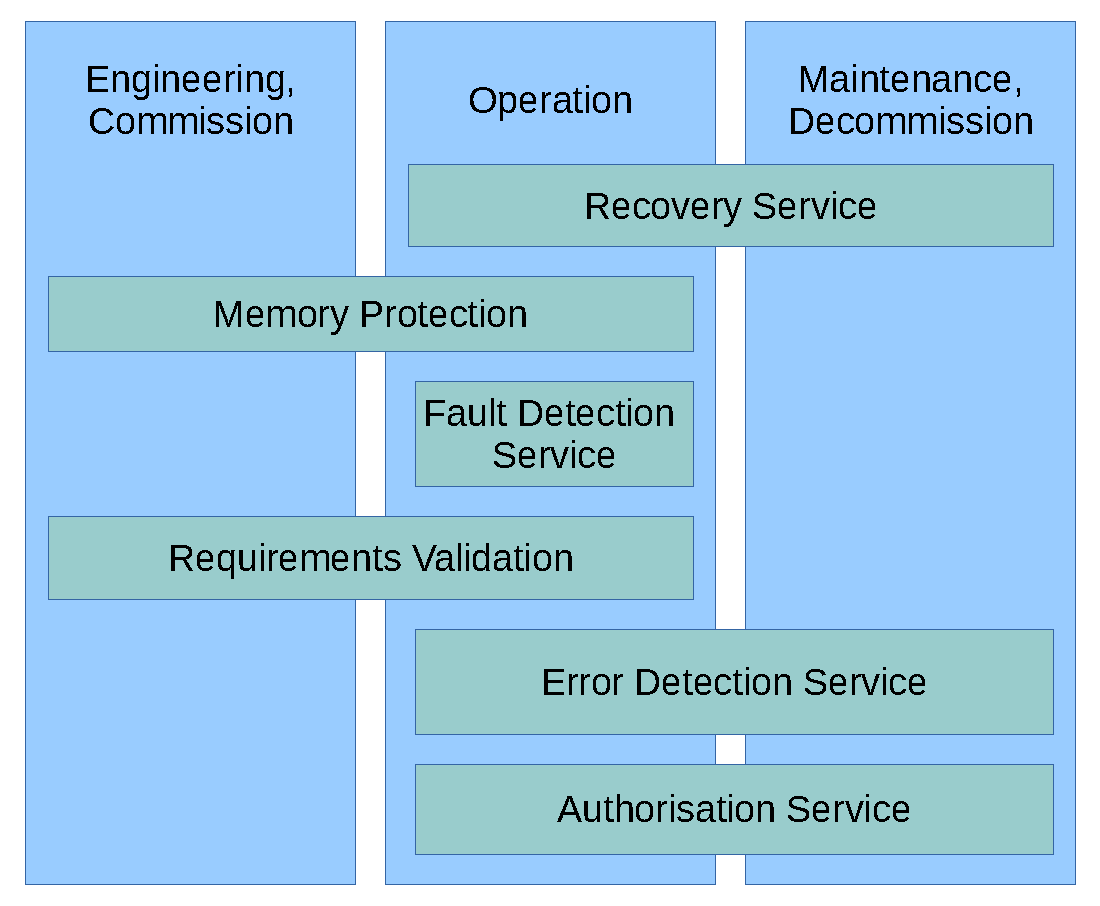
\includegraphics[scale=0.7]{safety-services-system-lifecycle.pdf}
\label{fig:safety-services-system-lifecycle}
\caption{Allocation of the safety service to the different system lifecycle phases.}
\end{figure}







\section{Service development process (use case scenario)}
\label{sec:service-development-process}

The preceding chapters analysed the concepts of SoA in embedded systems and safety services from a theoretical point of view. This final chapter investigates the design process of a safety-critical service by means of a simple use case. In detail, an \emph{error detection service}, based on triple modular redundancy, as it is presented in section \ref{sec:error-detection-service}, serves as example.

The considered development stages for this service are an adoption of the development stages, provided by Erl, Bennett et al. in \cite[p.116]{erl2011}. In detail, the first four stages are the object of investigation. Because the development of a single service is considered, instead of the development of a whole SoA, those stages are renamed:
\begin{itemize}
\item Service investigation/planning,
\item Service inventory analysis,
\item Service oriented analysis and
\item Service oriented design \cite[p.116]{erl2011}.
\end{itemize}

Each of the following four sections deals with one phase. They start off with a general description on what is conducted during this stage, before the example service is considered in this respect.




\subsection{Service investigation/planning}
This initial phase is concerned with the initial layout of the service. It is the phase where necessary requirements are listed and explored. There are several questions which need to be answered during this stage:
\begin{itemize}
\item What is the scope of the service?
\item What are required capabilities?
\item Which capabilities are not required?
\item What are the safety requirements concerning this service?
\item Should this functionality be implemented as service?
\end{itemize}



\subsection{Service inventory analysis}
The service inventory includes all services which could be provided by the vehicle. The difference to the service repository is that the service do not need to be available, or even implemented, but it is a static list of possible services.

During the \emph{service inventory analysis} the inventory is searched for services which are required in order to build up the desired service. This simplifies the development, because much of the required functionality is already provided by other services and at the same time this step is responsible for preventing redundancies.




\subsection{service oriented analysis}

The outcome of the \emph{service inventory analysis} phase is a so called \emph{service candidate}. This denotes a conceptual service model before it is implemented by means of a specific language. According to \cite[p.42]{erl2011}, the concept of a language independent service candidate is applied, because the service undergoes a lot of changes in these early stages of development. Nevertheless, this may not be practicable in reality. It is not unlikely that the service templates (provided by Arrowhead) are used and extended from the very beginning of the development process.

During the \emph{service oriented analysis} the service candidate is reviewed and checked with respect to \emph{naming} and \emph{normalisation}.

\begin{description}
	\item [Service naming] .
	The naming of the service candidate must be in accordance with other, existing services \cite[p.206]{erl2011}.

	In terms of automotive, the naming is governed by certain standards, like AUTOSAR, which proposes naming conventions in \textbf{SW-C and System Modelling Guide} \cite{autosar_system_modelling}.

	A unified naming convention is quite helpful, when dealing with standardised interfaces. It also provides the possibility to include relevant meta data into the name \cite{rehner2013}.

	\item [Service normalisation] .
	Services within the same \emph{service inventory} shall not have overlapping boundaries. In other words, redundant logic should generally be avoided, for it would violate the concept of a service oriented architecture. Accordingly, the services are forced to use existing services if those offer the required functionality \cite[p.207]{erl2011}.

	\item [Service Candidate Review] .
	The final phase of this stage is a review by the related developers. A possible outcome of this review is the approval of changes or extensions to the service candidate \cite[p.210]{erl2011}.

	In order to ensure an unbiased outcome, this review could be conducted by ``external'' people, which have not been included into the development process up to this step, but have a thorough knowledge of the SoA principles. Those people might think of a quite different approach for the same very same problem. This could raise new questions concerning the proposed design and composition.

	A review can also take place if an existing and already implemented service is extended by one or more new capabilities \cite[p.210]{erl2011}.
\end{description}




\subsection{service oriented design}

Erl, Bennett at al. describe this phase as:
\begin{quote}
\emph{``Service-Oriented Design subjects this service candidate to additional considerations that shape it into a technical service contract in alignment with other service contracts being produced for the same service inventory''} - \cite[p.86]{erl2011}.
\end{quote}


The aim of the \emph{service oriented design} is to physically establish the service contract by filling out the corresponding templates. It is initiated when sufficient analysis has been conducted.